\hypertarget{wsgi-ux63a5ux53e3}{%
\subsection{WSGI 接口}\label{wsgi-ux63a5ux53e3}}

了解了 HTTP 协议和 HTML 文档,我们其实就明白了一个 Web 应用的本质就是:

\begin{enumerate}
\def\labelenumi{\arabic{enumi}.}
\item
  浏览器发送一个 HTTP 请求;
\item
  服务器收到请求,生成一个 HTML 文档;
\item
  服务器把 HTML 文档作为 HTTP 响应的 Body 发送给浏览器;
\item
  浏览器收到 HTTP 响应,从 HTTP Body 取出 HTML 文档并显示。
\end{enumerate}

所以,最简单的 Web 应用就是先把 HTML 用文件保存好,用一个现成的 HTTP
服务器软件,接收用户请求,从文件中读取
HTML,返回。Apache、Nginx、Lighttpd
等这些常见的静态服务器就是干这件事情的。

如果要动态生成 HTML,就需要把上述步骤自己来实现。不过,接受 HTTP
请求、解析 HTTP 请求、发送 HTTP
响应都是苦力活,如果我们自己来写这些底层代码,还没开始写动态 HTML
呢,就得花个把月去读 HTTP 规范。

正确的做法是底层代码由专门的服务器软件实现,我们用 Python 专注于生成
HTML 文档。因为我们不希望接触到 TCP 连接、HTTP
原始请求和响应格式,所以,需要一个统一的接口,让我们专心用 Python 编写
Web 业务。

这个接口就是 WSGI:Web Server Gateway Interface。

WSGI 接口定义非常简单,它只要求 Web 开发者实现一个函数,就可以响应 HTTP
请求。我们来看一个最简单的 Web 版本的 ``Hello, web!'':

\begin{pythoncode}
def application(environ, start_response):
    start_response('200 OK', [('Content-Type', 'text/html')])
    return [b'<h1>Hello, web!</h1>']
\end{pythoncode}

上面的\texttt{application()}函数就是符合 WSGI 标准的一个 HTTP
处理函数,它接收两个参数:

\begin{itemize}
\item
  environ:一个包含所有 HTTP 请求信息的\texttt{dict}对象;
\item
  start\_response:一个发送 HTTP 响应的函数。
\end{itemize}

在\texttt{application()}函数中,调用:

\begin{pythoncode}
start_response('200 OK', [('Content-Type', 'text/html')])
\end{pythoncode}

就发送了 HTTP 响应的 Header,注意 Header
只能发送一次,也就是只能调用一次\texttt{start\_response()}函数。\texttt{start\_response()}函数接收两个参数,一个是
HTTP 响应码,一个是一组\texttt{list}表示的 HTTP Header,每个 Header
用一个包含两个\texttt{str}的\texttt{tuple}表示。

通常情况下,都应该把\texttt{Content-Type}头发送给浏览器。其他很多常用的
HTTP Header 也应该发送。

然后,函数的返回值\texttt{b\textquotesingle{}\textless{}h1\textgreater{}Hello,\ web!\textless{}/h1\textgreater{}\textquotesingle{}}将作为
HTTP 响应的 Body 发送给浏览器。

有了 WSGI,我们关心的就是如何从\texttt{environ}这个\texttt{dict}对象拿到
HTTP 请求信息,然后构造 HTML,通过\texttt{start\_response()}发送
Header,最后返回 Body。

整个\texttt{application()}函数本身没有涉及到任何解析 HTTP
的部分,也就是说,底层代码不需要我们自己编写,我们只负责在更高层次上考虑如何响应请求就可以了。

不过,等等,这个\texttt{application()}函数怎么调用?如果我们自己调用,两个参数\texttt{environ}和\texttt{start\_response}我们没法提供,返回的\texttt{bytes}也没法发给浏览器。

所以\texttt{application()}函数必须由 WSGI 服务器来调用。有很多符合 WSGI
规范的服务器,我们可以挑选一个来用。但是现在,我们只想尽快测试一下我们编写的\texttt{application()}函数真的可以把
HTML 输出到浏览器,所以,要赶紧找一个最简单的 WSGI 服务器,把我们的 Web
应用程序跑起来。

好消息是 Python 内置了一个 WSGI 服务器,这个模块叫 wsgiref,它是用纯
Python 编写的 WSGI 服务器的参考实现。所谓 ``参考实现''
是指该实现完全符合 WSGI
标准,但是不考虑任何运行效率,仅供开发和测试使用。

\hypertarget{ux8fd0ux884c-wsgi-ux670dux52a1}{%
\subsubsection{运行 WSGI 服务}\label{ux8fd0ux884c-wsgi-ux670dux52a1}}

我们先编写\texttt{hello.py},实现 Web 应用程序的 WSGI 处理函数:

\begin{pythoncode}
def application(environ, start_response):
    start_response('200 OK', [('Content-Type', 'text/html')])
    return [b'<h1>Hello, web!</h1>']
\end{pythoncode}

然后,再编写一个\texttt{server.py},负责启动 WSGI
服务器,加载\texttt{application()}函数:

\begin{pythoncode}
from wsgiref.simple_server import make_server

from hello import application
httpd = make_server('', 8000, application)
print('Serving HTTP on port 8000...')

httpd.serve_forever()
\end{pythoncode}

确保以上两个文件在同一个目录下,然后在命令行输入\texttt{python\ server.py}来启动
WSGI 服务器:

 
 \begin{figure}[htp]
	\centering
	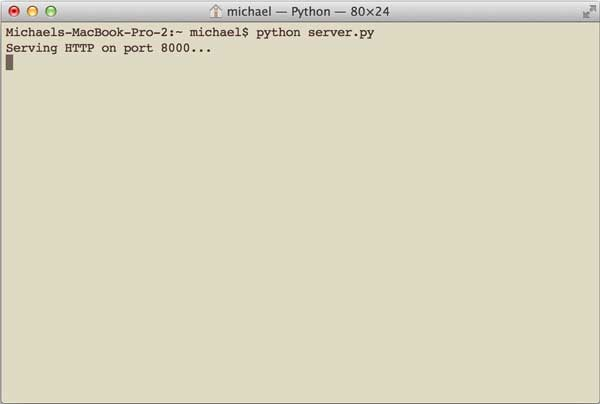
\includegraphics[width=0.6\linewidth]{fig/950751913543456.png}
\end{figure}


注意:如果\texttt{8000}端口已被其他程序占用,启动将失败,请修改成其他端口。

启动成功后,打开浏览器,输入\texttt{http://localhost:8000/},就可以看到结果了:

 
 \begin{figure}[htp]
	\centering
	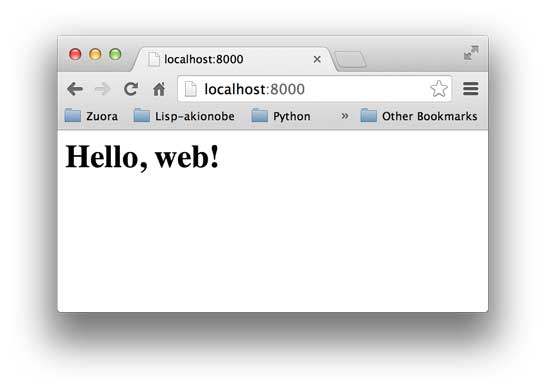
\includegraphics[width=0.6\linewidth]{fig/950751878708448.png}
\end{figure}


在命令行可以看到 wsgiref 打印的 log 信息:

 
 \begin{figure}[htp]
	\centering
	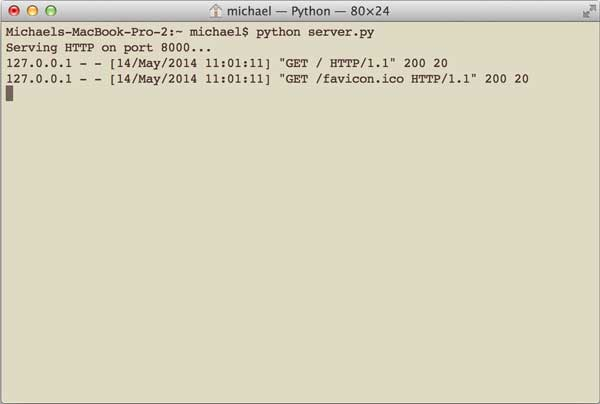
\includegraphics[width=0.6\linewidth]{fig/950751840957632.png}
\end{figure}


按\texttt{Ctrl+C}终止服务器。

如果你觉得这个 Web
应用太简单了,可以稍微改造一下,从\texttt{environ}里读取\texttt{PATH\_INFO},这样可以显示更加动态的内容:

\begin{pythoncode}
def application(environ, start_response):
    start_response('200 OK', [('Content-Type', 'text/html')])
    body = '<h1>Hello, %s!</h1>' % (environ['PATH_INFO'][1:] or 'web')
    return [body.encode('utf-8')]
\end{pythoncode}

你可以在地址栏输入用户名作为 URL 的一部分,将返回\texttt{Hello,\ xxx!}:

 
 \begin{figure}[htp]
	\centering
	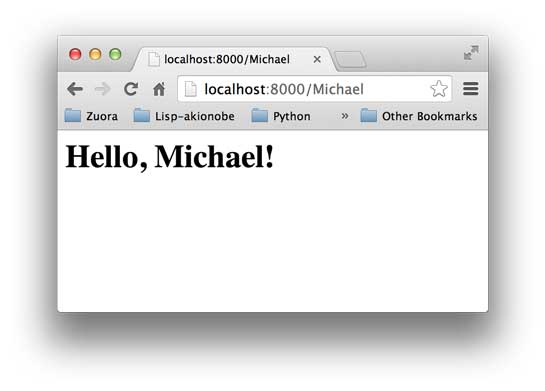
\includegraphics[width=0.6\linewidth]{fig/950751959286720.png}
\end{figure}


是不是有点 Web App 的感觉了?

\hypertarget{ux5c0fux7ed3}{%
\subsubsection{小结}\label{ux5c0fux7ed3}}

无论多么复杂的 Web 应用程序,入口都是一个 WSGI 处理函数。HTTP
请求的所有输入信息都可以通过\texttt{environ}获得,HTTP
响应的输出都可以通过\texttt{start\_response()}加上函数返回值作为 Body。

复杂的 Web 应用程序,光靠一个 WSGI 函数来处理还是太底层了,我们需要在
WSGI 之上再抽象出 Web 框架,进一步简化 Web 开发。

\hypertarget{ux53c2ux8003ux6e90ux7801}{%
\subsubsection{参考源码}\label{ux53c2ux8003ux6e90ux7801}}

\href{https://github.com/michaelliao/learn-python3/blob/master/samples/web/hello.py}{hello.py}

\href{https://github.com/michaelliao/learn-python3/blob/master/samples/web/do_wsgi.py}{do\_wsgi.py}

